\documentclass[14pt,a4paper]{extarticle}
\usepackage{fontspec}
\setmainfont{Times New Roman}
\usepackage[english,russian]{babel}
\usepackage{graphicx} % Required for inserting images
\usepackage[top=20mm,bottom=20mm,left=30mm,right=15mm]{geometry}
\usepackage{xcolor}
\usepackage{setspace}
\usepackage{tabularx}
\usepackage{fancyhdr}
\usepackage{caption}
\usepackage{graphicx}
\usepackage{placeins}
\usepackage{caption}
\usepackage{subcaption}
\usepackage{amsmath}
\usepackage{float}

\setlength{\parindent}{15mm}
\setstretch{1.5}
\linespread{1.25}
\tolerance=1
\emergencystretch=\maxdimen
\hyphenpenalty=10000
\exhyphenpenalty=10000
\usepackage{titlesec}
\titleformat{\section}[hang]{\normalfont\bfseries}{\thesection}{}{}
\titlespacing{\section}{15mm}{0pt}{0pt}
\captionsetup[figure]{name = {Рисунок}, labelsep = endash}

\begin{document}
\begin{titlepage}
    \begin{center}
    {\bfseries
    МИНОБРНАУКИ РОССИИ \\ САНКТ-ПЕТЕРБУРГСКИЙ ГОСУДАРСТВЕННЫЙ \\ ЭЛЕКТРОТЕХНИЧЕСКИЙ УНИВЕРСИТЕТ \\ <<ЛЭТИ>> ИМ. В.И. УЛЬЯНОВА (ЛЕНИНА)\\Кафедра САПР \vspace{0.23\textheight}
    
    ОТЧЕТ \\ по практической работе №7 \\ по дисциплине <<Информационные технологии>> \\ Тема: Вектора и матрицы. Градиент. \\
    \vspace{0.28\textheight}
        }
        \begin{table}[h!]
            \begin{tabularx}{\textwidth}{p{60mm}X>{\centering\arraybackslash}p{45mm}}
                Студент гр. 4352 & \_\_\_\_\_\_\_\_\_\_\_\_\_\_\_\_\_\_\_\_ & {Колесникова М. А.} \\ [5.4mm]  
                Преподаватель    & \_\_\_\_\_\_\_\_\_\_\_\_\_\_\_\_\_\_\_\_ & {Копец Е. Е.} \\ [5.4mm]
            \end{tabularx}
        \end{table}
    Санкт-Петербург\par
        2025
    \end{center}
\end{titlepage}
\setcounter{page}{2}

\section*{Цель работы.}

Научиться выполнять операции над векторами и матрицами, а также находить градиент.

\section*{Основные теоретические положения.}

В первом задании нужно сложить векторы, складывать векторы можно только одной размерности.\\
1. \[\begin{pmatrix} 1 & 2 & 3 & 4 \end{pmatrix} + \begin{pmatrix} 5 & 6 & 7 & 8 & 9 \end{pmatrix}\]
-- операция невозможна, так как не совпадает количество элементов ($4 \neq 5$);\\
2. \[\begin{pmatrix} 1 & 2 & 3 & 4 \end{pmatrix} + \begin{pmatrix} 10 & 11 & 12 & 13 \end{pmatrix} = \begin{pmatrix} 11 & 13 & 15 & 17 \end{pmatrix};\]\\
3. \[\begin{pmatrix} 1 & 2 & 3 & 4 \end{pmatrix} + \begin{pmatrix} 1 \\ 2 \\ 3 \\ 4 \end{pmatrix}\]
-- операция сложения невозможна, так как вектор-строка и вектор-столбец не совместимы;\\
4. \[\begin{pmatrix} 15 \\ 16 \\ 17 \\ 18 \\ 19 \end{pmatrix} + \begin{pmatrix} 3 \\ 3 \\ 3 \\ 3 \\ 3 \end{pmatrix} = \begin{pmatrix} 18 \\ 19 \\ 20 \\ 21 \\ 22 \end{pmatrix};\]
5. \[\begin{pmatrix} 15 \\ 16 \\ 17 \\ 18 \\ 19 \\ 21 \end{pmatrix} + \begin{pmatrix} 3 \\ 3 \\ 3 \\ 3 \\ 3 \end{pmatrix}\]
-- операция невозможна, так как не совпадает количество элементов ($6 \neq 5$).\\

Во втором задании нужно найти значения выражений.\\
1. \[5\times\begin{pmatrix} 1 & 2 & 3 & 4 & 5 & 6 \end{pmatrix}-3\times\begin{pmatrix} 5 & 6 & 7 & 8 & 9 & 10 \end{pmatrix} = \begin{pmatrix} -10 & -8 & -6 & -4 & -2 & 0 \end{pmatrix};\]
2. \[12\times\begin{pmatrix} 7 & 12 & 11 & 14 & 9 & 16 & 21 \end{pmatrix}-3.2\times\begin{pmatrix} 13 & 61 & 24 & 76 & 1 & 3 & 8 \end{pmatrix} =\]
\[=\begin{pmatrix} 42.4 & -51.2 & 55.2 & -75.2 & 104.8 & 182.4 & 226.4 \end{pmatrix};\]
3. \[7\times\begin{pmatrix} 15 \\ 16 \\ 17 \\ 18 \\ 19 \end{pmatrix}+\frac{1}{3}\times\begin{pmatrix} 3 \\ 3 \\ 3 \\ 3 \\ 3 \end{pmatrix}
=\begin{pmatrix} 106 \\ 113 \\ 120 \\ 127 \\ 134 \end{pmatrix};\]
4. \[7\times\begin{pmatrix} 11 \\ 21 \\ 78 \\ 32 \\ 2 \end{pmatrix}-\frac{2}{5}\times\begin{pmatrix} 5 \\ 6 \\ 7 \\ 9 \\ 3 \end{pmatrix}
=\begin{pmatrix} 75 \\ 
    144.6 \\ 
    543.2 \\ 
    220.4 \\ 
    12.8 \end{pmatrix};\]

В третьем задании нужно найти скалярное произведение векторов, если операция имеет смысл.\\
1. \[\begin{pmatrix} 1 & 2 & 3 & 4 & 5 \end{pmatrix}\times\begin{pmatrix} 5 & 6 & 7 & 8 & 9 \end{pmatrix} = 5 + 12 + 21 + 32 + 45 = 115;\]
2. \[\begin{pmatrix} 4 & 3 & 8 & 12 & 1 \end{pmatrix}\times\begin{pmatrix} 3 & 2 & 13 & 8 & 5 \end{pmatrix} = 12 + 6 + 104 + 96 + 5 = 223;\]
3. \[\begin{pmatrix} 1 & 2 & 3 & 4 \end{pmatrix}\times\begin{pmatrix} 5 & 6 & 7 & 8 & 9 \end{pmatrix}\]
-- векторы нельзя скалярно перемножить, так как у них разная размерность ($4 \neq 5$).

В четвёртом задании нужно транспонировать матрицы. Для нужно их как бы повернуть (поменять строки и столбы местами).\\
1. Транспонирование вектора-строки:
\[
(5\ 6\ 7\ 8\ 9)^T = \begin{pmatrix} 5 \\ 6 \\ 7 \\ 8 \\ 9 \end{pmatrix};\]
2. Транспонирование вектора-столбца:
\[
\begin{pmatrix}
5 \\
6 \\
7 \\
8 \\
9
\end{pmatrix}^T = (5\ 6\ 7\ 8\ 9);\]
3. Транспонирование матрицы $4\times4$:
\[
\begin{pmatrix}
1 & 2 & 3 & 4 \\
5 & 6 & 7 & 8 \\
9 & 10 & 11 & 12 \\
13 & 14 & 15 & 16
\end{pmatrix}^T = 
\begin{pmatrix}
1 & 5 & 9 & 13 \\
2 & 6 & 10 & 14 \\
3 & 7 & 11 & 15 \\
4 & 8 & 12 & 16
\end{pmatrix};
\]

Транспонирование матрицы можно запрограммировать с помощью sympy (рис. \ref{pic:trans}).

\begin{figure}[h!]
    \centering
    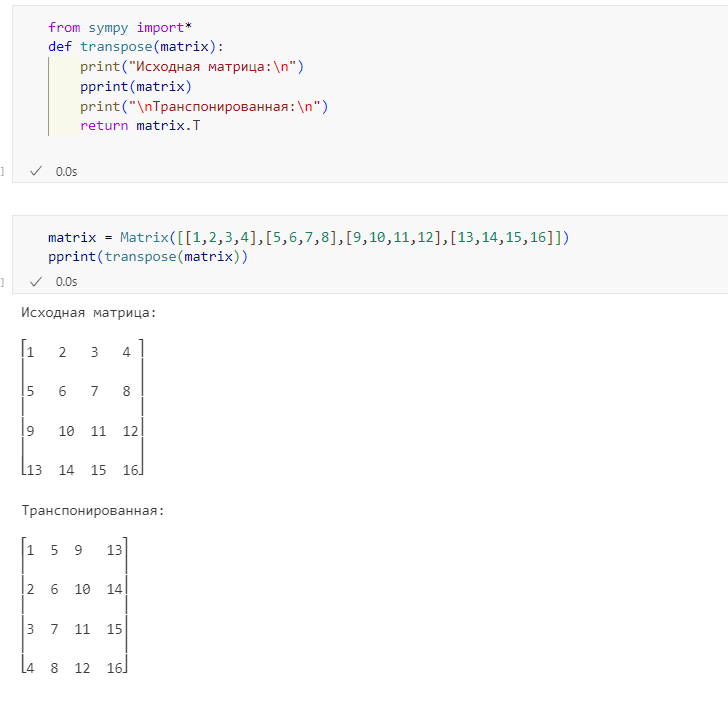
\includegraphics[scale=0.7]{pic7/trans.png}
    \caption{Нахождение транспонированной матрицы}
    \label{pic:trans}
\end{figure}
\FloatBarrier

Складывать векторы можно по правилу треугольника:
начало одного из векторов переносится в конец другого (на рисунках выделен красным пунктиром),
затем рисуется вектор из начала первого вектора (на рисунках выделен фиолетовым).
Векторы с рисунков можно проверить посчитав выражения:\\
а. $2 \cdot (1 \ 0) + 3 \cdot (0 \ 1) = (2 \ 0)+(0 \ 3)=(2 \ 3)$. Значение совпадает с геометрическим (рис. \ref{pic:a}).
\begin{figure}[h!]
    \centering
    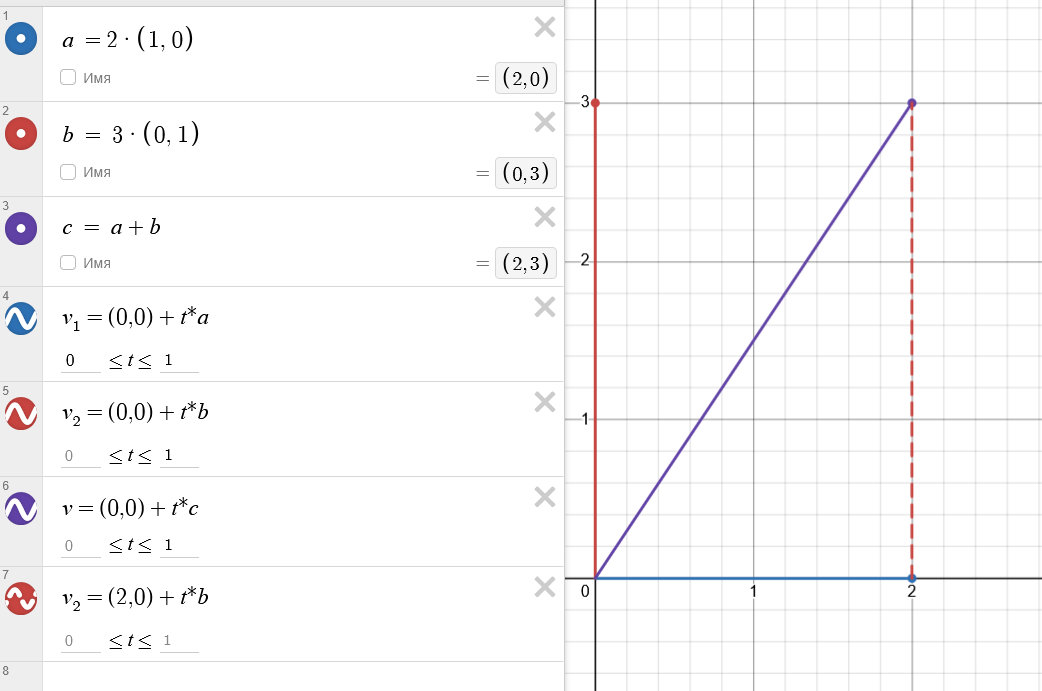
\includegraphics[scale=0.5]{pic7/5.a.png}
    \caption{Сложение векторов $2 \cdot (1 \ 0) + 3 \cdot (0 \ 1)$}
    \label{pic:a}
\end{figure}
\FloatBarrier
b. $3 \cdot (1 \ 2) + 2 \cdot (0 \ 1) = (3 \ 6)+(0 \ 2)=(3 \ 8)$. Значение совпадает с геометрическим (рис. \ref{pic:b}).
\begin{figure}[h!]
    \centering
    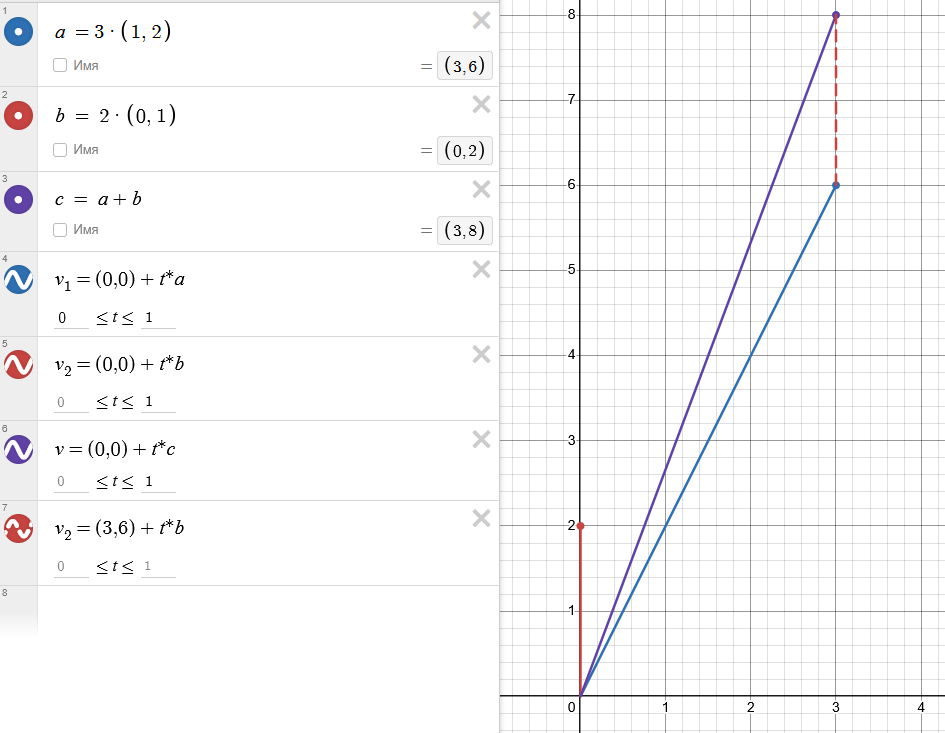
\includegraphics[scale=0.5]{pic7/5.b.png}
    \caption{Сложение векторов $3 \cdot (1 \ 2) + 2 \cdot (0 \ 1)$}
    \label{pic:b}
\end{figure}
\FloatBarrier
c. $2 \cdot (2 \ 3) + (3 \ 4) = (4 \ 6)+(3 \ 4)=(7 \ 10)$. Значение совпадает с геометрическим (рис. \ref{pic:c}).
\begin{figure}[h!]
    \centering
    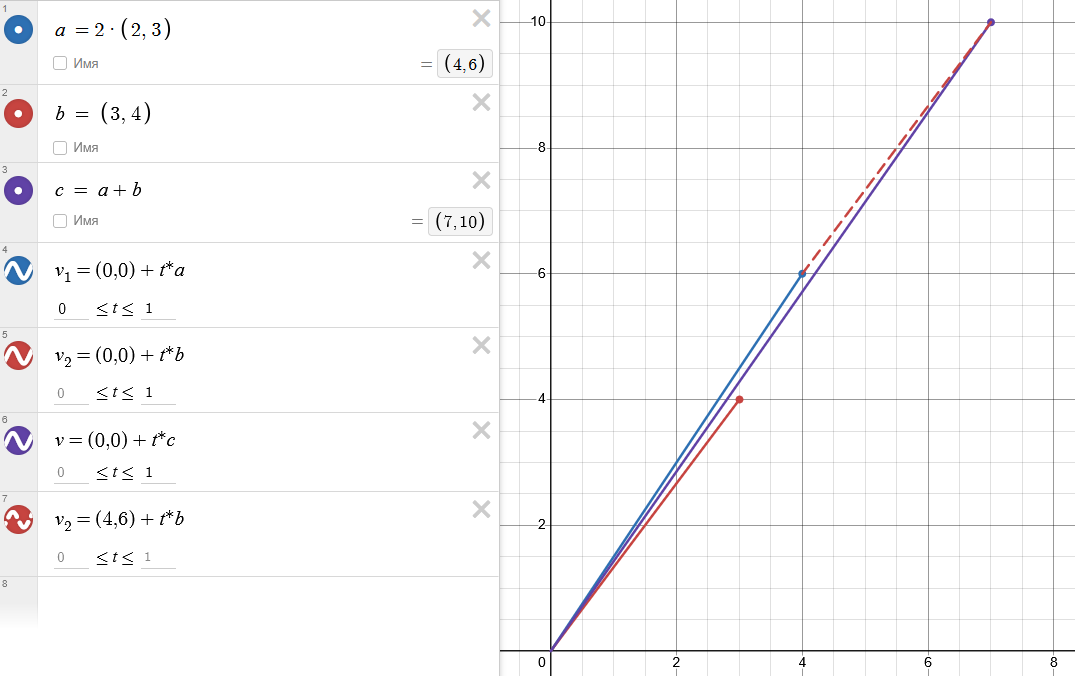
\includegraphics[scale=0.5]{pic7/5.c.png}
    \caption{Сложение векторов $2 \cdot (2 \ 3) + (3 \ 4)$}
    \label{pic:c}
\end{figure}
\FloatBarrier

Для следующего задания найдём аналитически значение,
а затем построим график.\\
a. $2 \cdot (1 \ 0 \ 0) + 3 \cdot (0 \ 1 \ 0) + (0 \ 0 \ 1) = (2 \ 3 \ 1)$;\\
b.	$(2 \ 3 \ 4) + 2 \cdot (1 \ 1 \ 1) = (4 \ 5 \ 6)$\\
Для сложения также используется правило треугольника, но также нужно поднять
вектор на ещё одно измерение, которое на рисунках выделено серым (рис. \ref {pic:a2}, \ref {pic:b2}).
\begin{figure}[h!]
    \centering
    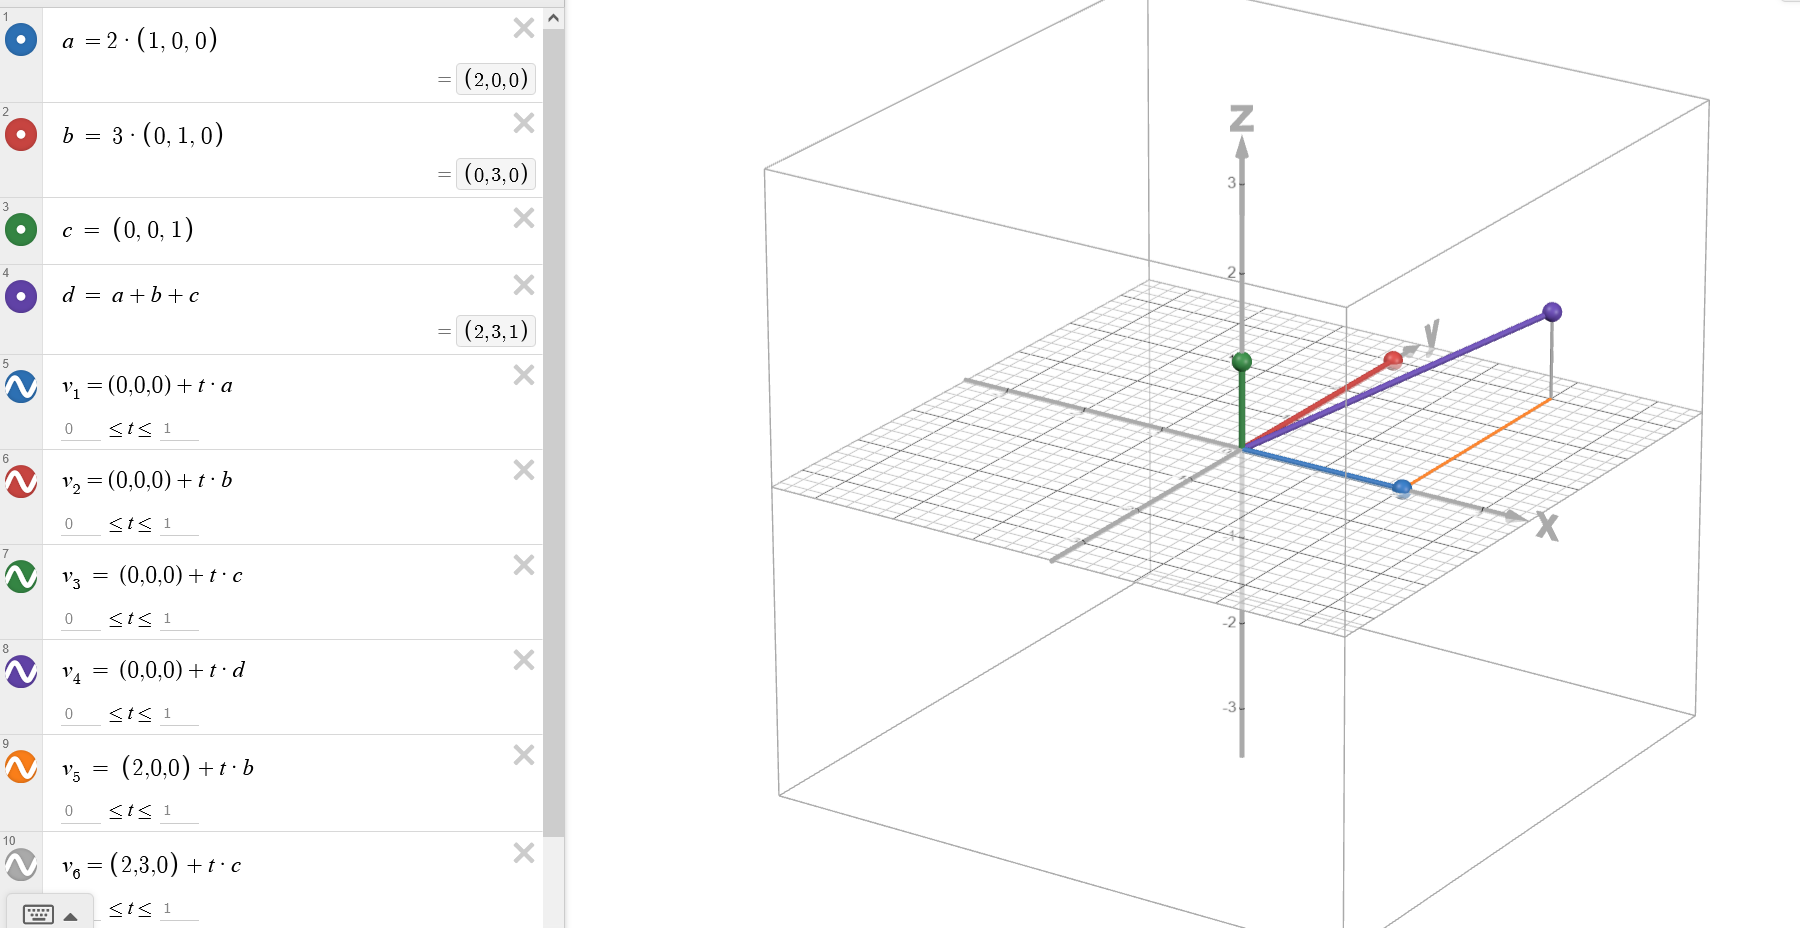
\includegraphics[scale=0.3]{pic7/5.3.a.png}
    \caption{Сложение векторов $2 \cdot (1 \ 0 \ 0) + 3 \cdot (0 \ 1 \ 0) + (0 \ 0 \ 1)$}
    \label{pic:a2}
\end{figure}
\FloatBarrier
\begin{figure}[h!]
    \centering
    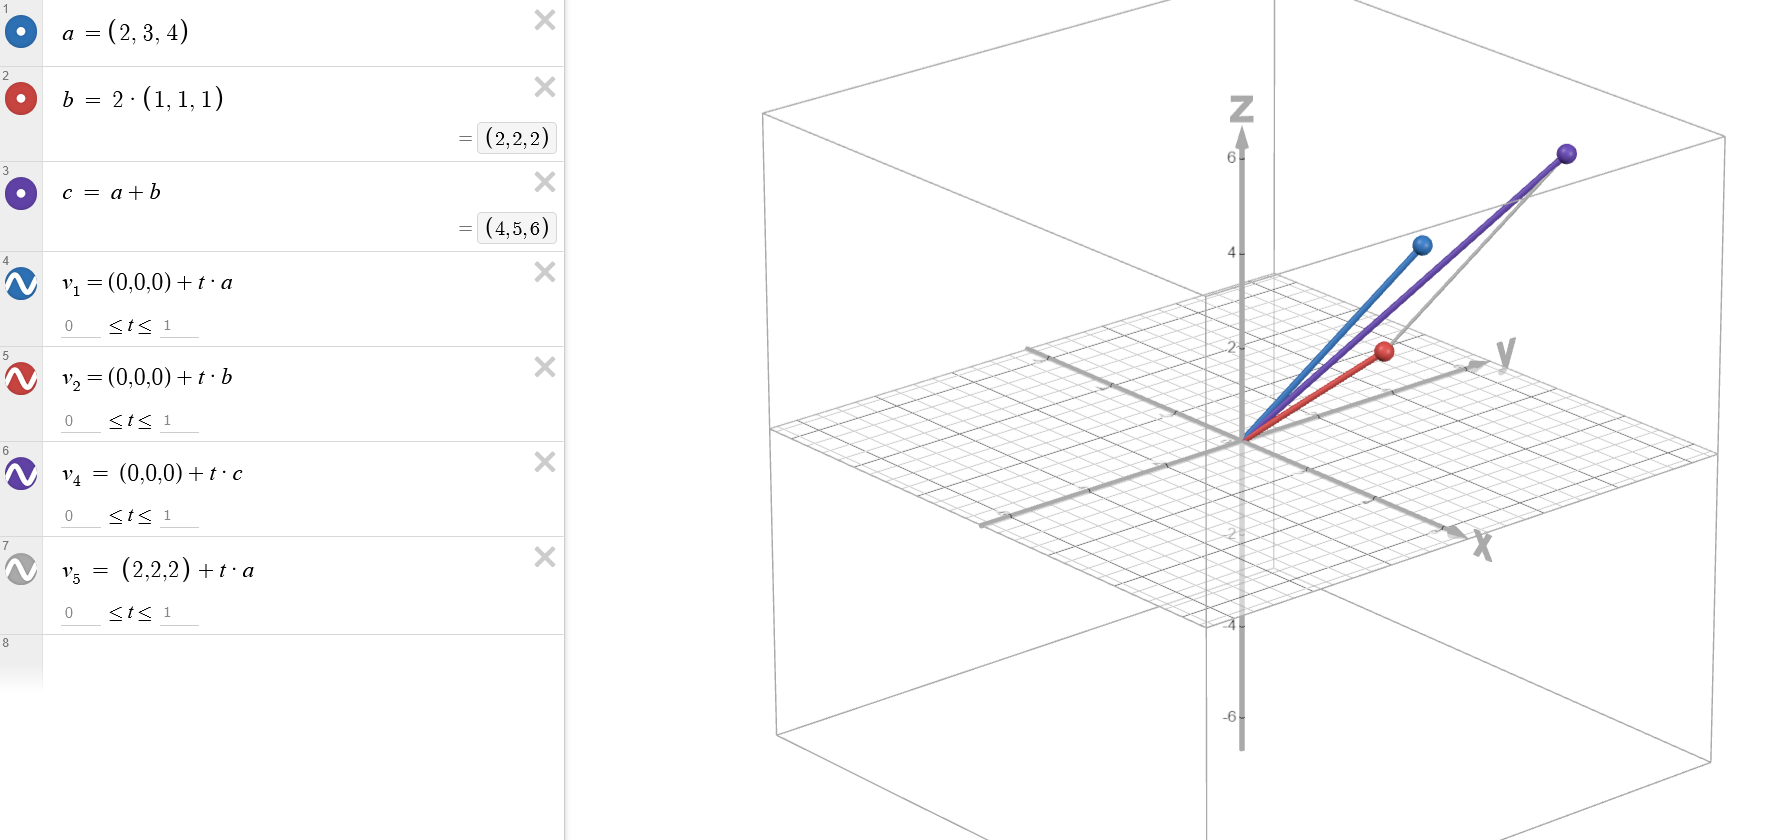
\includegraphics[scale=0.3]{pic7/5.3.b.png}
    \caption{Сложение векторов $(2 \ 3 \ 4) + 2 \cdot (1 \ 1 \ 1)$}
    \label{pic:b2}
\end{figure}
\FloatBarrier

В следующем задании нужно умножить векторы на константы, а затем скалярно перемножить полученные векторы.\\
1. \[3 \times(2 \ 5 \ 0 \ 6 \ 8 \ 10 \ 6 \ 7 \ 5 \ 7) \cdot 2 \times (8 \ 6 \ 7 \ 9 \ 6 \ 6 \ 2 \ 3 \ 2 \ 3) =\]
\[= (6 \ 15 \ 0 \ 18 \ 24 \ 30 \ 18 \ 21 \ 15 \ 21) \cdot (16 \ 12 \ 14 \ 18 \ 12 \ 12 \ 4 \ 6 \ 4 \ 6) =\]
\[= 96 + 180 + 0 + 324 + 288 + 360 + 72 + 126 + 60 + 126 = 1632;\]\\
2. 
\[6 \times (9 \ 6 \ 7 \ 7 \ 0 \ 1 \ 6 \ 8 \ 1 \ 2) \cdot 5 \times (0 \ 2 \ 2 \ 6 \ 7 \ 8 \ 8 \ 3 \ 1 \ 8) =\]
\[= (54 \ 36 \ 42 \ 42 \ 0 \ 6 \ 36 \ 48 \ 6 \ 12) \cdot (0 \ 10 \ 10 \ 30 \ 35 \ 40 \ 40 \ 15 \ 5 \ 40) =\]
\[= 0 + 360 + 420 + 1260 + 0 + 240 + 1440 + 720 + 30 + 480 = 4950;\]\\
3. 
\[(2 \ 5 \ 0 \ 6 \ 8 \ 10 \ 6 \ 7 \ 5 \ 7) \cdot (8 \ 6 \ 7 \ 9 \ 6 \ 6 \ 2 \ 3 \ 2 \ 3) =\]
\[= 16 + 30 + 0 + 54 + 48 + 60 + 12 + 21 + 10 + 21 = 272;\]\\
4. 
\[(9 \ 6 \ 7 \ 7 \ 0 \ 1 \ 6 \ 8 \ 1 \ 2) \cdot (0 \ 2 \ 2 \ 6 \ 7 \ 8 \ 8 \ 3 \ 1 \ 8) =\]
\[= 0 + 12 + 14 + 42 + 0 + 8 + 48 + 24 + 1 + 16 = 165.\]

Для транспонирования матрицы нужно написать код, в котором
функция будет принимать и возвращать либо numpy.array, либо list (рис. \ref{pic:cod}).
Результат его работы представлен (рис. \ref{pic:rez}).
\begin{figure}[h!]
    \centering
    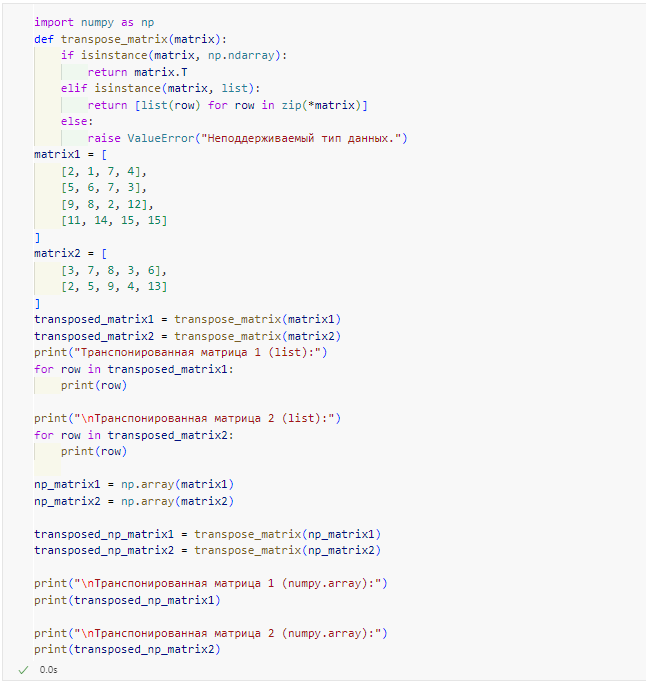
\includegraphics[scale=0.8]{pic7/cod.png}
    \caption{Код для транспонирование матриц}
    \label{pic:cod}
\end{figure}
\FloatBarrier
\begin{figure}[h!]
    \centering
    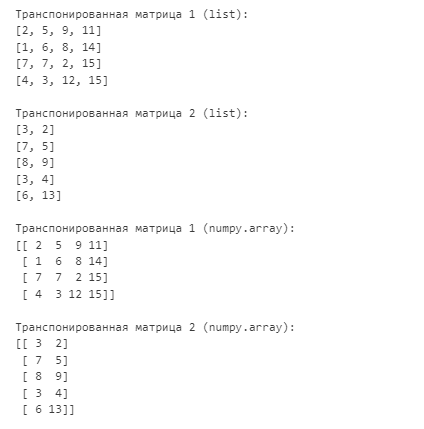
\includegraphics[scale=0.8]{pic7/rez.png}
    \caption{Транспонированные матрицы}
    \label{pic:rez}
\end{figure}
\FloatBarrier

В последнем задании нужно завершить градиентный спуск,
начатый в методических материалах. Движение будет происходить в направлении антиградиента,
размер шага равен $0.01$. В каждой новой точке антиградиент будет разным. Нужно добиться величины MSE меньше 6,36,
а также посчитать количество шагов градиентного спуска.

Функция потерь MSE:
\[{MSE}(a_1, a_2) = \frac{1}{4} ((a_1 + 2a_2 - 5)^2 + (5a_1 + 3a_2 - 6)^2 +\]\[+ (2a_1 + 4a_2 - 10)^2 +(3a_1 + 7a_2 - 8)^2).\]

Градиент MSE:
\[\nabla \text{MSE}(a_1, a_2) = \begin{pmatrix}19.5a_1 + 23a_2 - 39.5 \\ 23a_1 + 39a_2 - 62\end{pmatrix}.\]

Начальная точка: $(a_1, a_2) = (0.57, 0.91).$

Начальное значение MSE: $8.56.$

Вычисляем новое значение MSE (рис. \ref{pic:mse}). Значение меньше $6.36$ было достигнуто за 6 шагов.

\begin{figure}[h!]
    \centering
    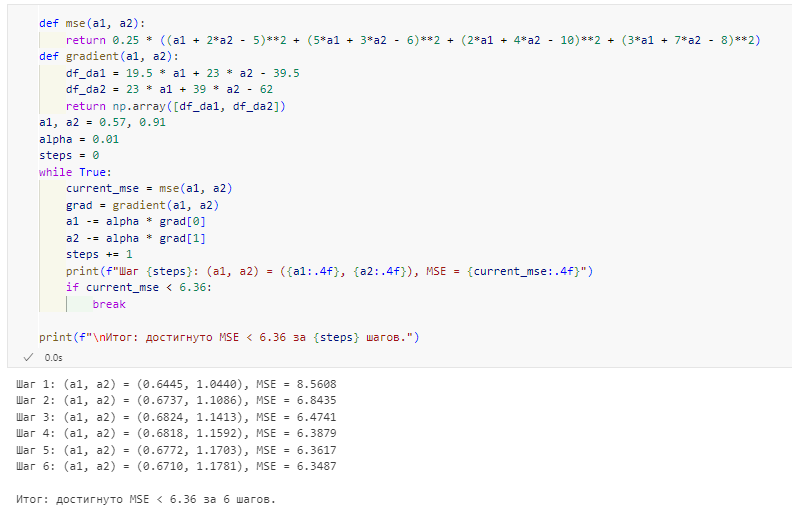
\includegraphics[scale=0.7]{pic7/mse.png}
    \caption{Поиск градиента меньшего $6.36$}
    \label{pic:mse}
\end{figure}
\FloatBarrier

\section*{Вывод.}

В ходе работы было изучено сложение векторов, умножение вектора на число, транспонирование матриц. А также нахождение
скалярного произведение векторов как аналитически, так и геометрически. Помимо этого было изучено нахождение
функции векторного аргумента и градиента.

\end{document}